\chapter{Restricting and ordering}\label{cha:restricting-ordering}

\minitoc

\section{Conditionals and modals}
\label{sec:conditionals-modals}

\note{Thus continues our ``chemistry'' experiments, combining expressions we
  have an initial theory about and seeing what happens when they are put in
  contact.}%
We have a basic theory of conditionals in place as well as a basic theory of
modals. Both are treated as intensional operators that move us from the initial
evaluation world to another set of worlds: in the case of conditionals, those
worlds where the antecedent is true that are otherwise relevantly like the
evaluation world; in the case of modals, to whatever worlds the contextually
supplied accessibility relation assigns to the evaluation world. This means that
if a sentence contains both a conditional and a modal, we expect them to work
together to express nested intensional shifting.

\subsection{First steps}

In many cases, the experiments seem to have the expected outcome. Consider the
following attempt to embed a modal in the antecedent of a conditional:

\ex
If one can get to that beach by bike, Iris did just that.
\xe
%
This seems to have the meaning we predict: the conditional take us to worlds
where a certain modal fact holds \dash that the beach is reachable by bike \dash
and then we say that in those worlds Iris went to the beach by bike.

\kwn Or consider our friend Howard again:

\ex If Howard has to pay a heavy fine, he will be broke. \xe
%
\note{In our system, this could be captured by saying that the context supplies
  an $f$ that assigns to the evaluation world only worlds where Howard does what
  he is obligated to, at least in as much as paying fines is concerned.}%
Note that by itself, being under the obligation to pay a fine doesn't
automatically mean that one does. So, \Last indirectly signals that if Howard
has to pay a heavy fine, he will comply and thus he will be broke.

One thing that lots of people think is not straightforwardly possible is
epistemic modals in conditionals antecedent. \cite{papafragou-2006-epistemic},
for example, finds the following examples problematic:

\pex
\a ?If Max must be lonely, his wife will be worried.
\a ?If Max may be lonely, his wife will be worried.
\xe
%
\note{What exactly we might mean by ``iffy'' and how exactly conditionals signal
  iffiness is an interesting question. Any ideas?}%
One possible explanation is that conditionals signal that the antecedent is
``iffy''. An epistemic modal statement can only be ``iffy'' if the speaker is
not certain about what ``the evidence'' is. That can only be if ``the evidence''
is not the evidence that the speaker has full access to. Relevant examples
include the ``cancer scenarios'' of \cite{derose-1991-epistemic} and the
``Mastermind'' cases of \cite{fintel-gillies-2007-ose2,fintel-gillies-2011-mmr}:
\marginfig{Mastermind.jpg}%

\pex
\a If John might have cancer [the doctors haven’t told us], he will have to see
an expert in Boston.
\a If there have to be two reds, your next move is obvious.
\xe
%
These seem to have acceptable readings where the conditional takes us to worlds
where the embedded epistemic modal claim holds.

Consider next modals in the consequent of conditionals. On the face of it,
examples abound:
%
\note{\Next[b] is from a term paper by Moss. \Next[c] is due to 
  Zvolenszky.}%
\pex
\a If jaywalking is illegal here, then that guy has to pay a fine.
\a If Caspar vacuums on Saturday, then Chris has to cook on Sunday.
\a If Britanny drinks Coke, she must drink Coke.
\a If Howard returns his book late, he has to pay a fine.
\a If Cosette has to be home by midnight, she ought to think about leaving
now.
\xe
%
We will see, however, that there are significant challenges for compositional
semantics hiding here. We begin with the interaction of epistemic modals and
conditionals. 

\clearpage
\subsection{A serious problem}
\label{subsec:problem}

\marginfig{map.png}%
Our friends have been driving in the Massachusetts hinterlands, inexplicably
without iPhones or GPS, and are relying entirely on an old-fashioned map.
They've just passed through a little town with an iconic New England church and
are looking on the map to try to figure out where they are. They have concluded
that they are either on Route 117 or on Route 62. There are two plausible
candidate towns on Route 117 (Maynard and Stow) and just one on Route 62
(Hudson).

So, given all the evidence available to them, there are three live
possibilities: that they are in Hudson (on Rte 62, and they don't know it), that
they are in Stow (on Rte 117, and they don't know it), and that they are in
Maynard (on Rte 117, and they don't know it).

It's true when they say:

\ex We might be in Maynard.\xe
%
since there are worlds compatible with their evidence where they are in
Maynard.

\kwn It's true when they say:

\ex If we're on Route 62, we're in Hudson.\label{ex:bare-hudson}\xe
%
because of the three towns that they know they might be in, only Hudson
is on Rte 62.

Our semantics for conditionals has the conditional take us to worlds that are
(i) in $f(w)$, here in the set of worlds compatible with their evidence and (ii)
are antecedent worlds. Among the worlds compatible with their evidence, all
$p$-worlds (worlds where they are in Rte 62) are worlds where they are in
Hudson.

So far so good. But here are some problematic cases (with the intuitive
truth-value judgments in the given scenario):

\pex\label{ex:trouble}%
\a If we're on Route 117, we might be in Stow. \hfill True
\a If we're on Route 117, we might be in Hudson.\hfill False
\a If we're on Route 62, we must be in Hudson.\hfill True
\xe
%
We will now see that these cannot be explained in our framework!

Take \Last[c] first. The conditional takes us to those worlds that are (i)
compatible with their evidence or with what they know (which includes their
knowledge that they don't know in which of the three towns they are) and (ii)
where they are on Rte 62. In all of those worlds, they are in Hudson, but in
none of them do they \emph{know} or \emph{have any additional evidence} that
they are in Hudson. So, we expect \Last[c] to be false, contrary to fact.

Now, take \Last[b]. We go to worlds compatible with their evidence where they
are on Route 117. All of them are worlds where they are on Route 117 without
knowing that they are there, since they know that they don't know where they
are. In those worlds, is it true that for all they know, they are in Hudson?
Yes. Therefore, we predict that \Last[b] is true, again contrary to fact.

Finally, while we do predict that \Last[a] is true, the reason is simply that
because of their ignorance, any world compatible with their evidence is a world
where any of the relevant \emph{might}-claims is true. So, the conditional
antecedent is predicted to make no difference to the truth of the epistemic
possibility claim in its consequent, contrary to fact (our intuitions are
different for \Last[a] vs. \Last[b]).

Before we turn to one of the dominant ways of accounting for the meanings of the
examples in \Last, let's consider a tempting idea about \Last[c]: what if the
epistemic necessity modal \emph{must} actually scopes over the conditional, even
though it appears in its consequent? At first glance, the resulting meaning is
not far off the target. The claim would be that in all the epistemically
accessible worlds the conditional \refx{ex:bare-hudson} \emph{if we're on Rte
  62, we're in Hudson} is true. We already saw that that conditional is true in
the actual world, and there's no reason to say that it isn't true in other
epistemically accessible worlds. So far, so good.

Unfortunately, there are several reasons for doubting that this LF with
wide-scope for the modal is a convincing solution to our troubles:

\begin{enumerate}
\item For the \emph{might}-version, we can't resort to wide-scoping the modal,
  because the epistemic conditional \emph{if we're on Rte 117, we're in Stow} is
  false in the actual world and in fact in all epistemically accessible worlds:
  they have evidence that entails that it doesn't follow from being on Rte 117
  that they're in Stow. So, \Last[a] would be predicted to be false under the
  wide-scope LF. So, no matter how we scope the modal, we either have trivial
  truth or falsity, and not what we want: non-trivial truth-conditions.

\item Epistemic \emph{must} carries with it an ``evidential signal''
  \parencite{fintel-gillies-2010-mss}:

  \ex It must be raining. \xe
%
  This signals that the speaker inferred the truth of \emph{it is raining}
  indirectly on the basis of other evidence. The signal is still perceptible
  when the prejacent is a generalization or conditional:

  \pex
  \a Elephants must dislike bees.
  \a George must have to be home by midnight.
  \a It must be that if they're on Rte 62, they are in Clinton.
  \xe
%
  But \refx[c]{ex:trouble} is not felt to have such a signal, other than that
  the antecedent would be an additional piece of information in the deduction
  that they're in Hudson.

\item We also need to be able to analyze epistemic conditionals with two modals
  in a conjunctive consequent (examples like this are discussed in
  \cite{gillies-2010-iffiness}):

  \ex\label{ex:two-modals} If we're on Rte 62, we must be in Hudson and might be
  very close to the Horseshoe pub. \xe
%
  A wide-scope analysis of the modals in \Last seems impossible.

\end{enumerate}
%
Conclusion: our analysis really is in trouble and can't be rescued by
wide-scoping.

In the next section, we present the dominant treatment of the interaction of
conditionals and modals in current linguistic semantics. There are alternatives
that deserve to be considered, but that would lead us beyond the bounds of this
textbook.

\subsection{\expression{If}-clauses as restrictors}

The problem we have encountered here with the interaction of an
\expression{if}-clause and the modal operator \expression{might} is similar to
others that have been noted in the literature. Most influentially, Lewis in his
paper ``Adverbs of Quantification'' \parencite{lewis-1975-adverbs} showed how
hard it is to find an adequate analysis of the interaction of
\expression{if}-clauses and \term{adverbs of quantification} like
\expression{never, rarely, sometimes, often, usually, always} in sentences like
these:

\ex \choice{Always,Usually,Often,Sometimes,Rarely,Never} if a driver sees a
friend walking, she offers her a ride. \xe
%
Lewis proposed that in these cases, the adverb is the only operator at work and
that the \expression{if}-clause serves to restrict the adverb. Thus, it has much
the same function that a common noun phrase has in a determiner-quantification.

\begin{quote}
	
	The \expression{if} of our restrictive \expression{if}-clauses should not be
  regarded as a sentential connective. It has no meaning apart from the adverb
  it restricts. The \expression{if} in \expression{always if \ldots, \ldots,
    sometimes if \ldots, \ldots}, and the rest is on a par with the
  non-connective \expression{and} in \expression{between \ldots and \ldots},
  with the non-connective \expression{or} in \expression{whether \ldots or
    \ldots}, or with the non-connective \expression{if} in \expression{the
    probability that \ldots if \ldots}. It serves merely to mark an
  argument-place in a polyadic construction. \parencite[11]{lewis-1975-adverbs}

\end{quote}
%
Building on Lewis' insight, Kratzer argued for a uniform treatment of
\expression{if}-clauses as restrictors. She claimed that

\begin{quote}
	
	the history of the conditional is the story of a syntactic mistake. There is
  no two-place \expression{if \ldots then} connective in the logical forms of
  natural languages. \expression{If}-clauses are devices for restricting the
  domains of various operators. \citep{kratzer-1986-conditionals}
\end{quote}
%
\kwn Let us repeat this:

\ex \extitle{Kratzer's Thesis}\\[3pt]
\expression{If}-clauses are devices for restricting the domains of various
operators.\xe

Kratzer's Thesis gives a unified picture of the semantics of conditional
clauses. Note that it is not meant to supplant previous accounts of the
\emph{meaning} of conditionals. It just says that what those accounts are
analyzing is not the meaning of \expression{if} itself but the meaning of the
operators that \expression{if}-clauses restrict.

Let us see how this idea helps us with our most problematic case,
\emph{\refx[c]{ex:trouble} If we're on Route 62, we must be in Hudson}. The idea
is to deny that there are two quantifiers over worlds in this sentence. Instead,
the \expression{if}-clause merely contributes a further restriction to the modal
\expression{must}. %
\note{Note that this is not the same as worlds where they are on Route 62
  \emph{and know that they are}. This is made vivid by examples ultimately due
  to Thomason (as noted in \cite{fraasen-1980-ellis-review}): \emph{If my
    partner is embezzling, I will never know (because I'm so bad at
    accounting)}.}%
In effect, the modal is not quantifying over \emph{all} the worlds compatible
with our friends' knowledge but only over those where they are on Route 62. It
then claims that all of those worlds are worlds where they are in Hudson. Since
that is in fact true, we now correctly predict that \refx[c]{ex:trouble} is
true. 

What we don't yet have is a compositional calculation. What does it mean in
structural terms for the \expression{if}-clause to be restricting the domain of
the modal? We present here a particularly ``flat-footed'' implementation. The
idea is that \emph{if}-clauses serve as modifiers of the modal flavor argument
of modals.

Recall the entry we had for \emph{must}:

\ex
$\svt{must}^{w,g} = \lambda f_{s,st}. \lambda p_{st}.\ \forall w'\co w'
\in f(w) \longrightarrow\ p(w') = 1$.
\xe
%
We supplied the modal with a covert ``pronoun'' of type \type{s,st} as its first
argument:

\ex
\begin{forest}
baseline,
sn edges,
for tree={s sep=10mm, inner sep=0, l=0}
[{}, my pretty nice empty nodes
[[must]
[$f_{3,\type{s,st}}$]
]
[[we be in Hudson, roof]]
]
\end{forest}
\xe
%
\kwn\enlargethispage{36pt}%
\noindent We assume a structure where the \emph{if}-clause is the sister of the
$f$-pronoun:

\ex
\begin{forest}
baseline,
sn edges,
for tree={s sep=10mm, inner sep=0, l=0}
[{}, my pretty nice empty nodes
[
[must]
[
[$f_{3,\type{s,st}}$]
[
[if]
[[we are on Rte 62, roof]]
]
]
]
[[we be in Hudson, roof]]
]
\end{forest}
\xe
%
\clearpage%
\note{This implementation of the restrictor theory was considered (and, without
  much of an argument, dismissed) in Section 3.2 of \cite{fintel-1994-thesis}
  and is also found in lecture notes from 2004 by von Stechow. In Section 3.3 of
  \cite{fintel-1994-thesis}, a different approach is developed, which is adopted
  (at least for illustration) by \cite{kratzer-2015-hook}. The idea is that
  \emph{if}-clauses are variable modifiers, something very like variable binders
  without entirely overwriting the current variable assignment. Further
  references about the restrictor theory are given at the end of this chapter.
}%
The idea now is that the two restrictive devices work together: we just feed to
the modal the \emph{intersection} of (i) the set of worlds that are
$f_{3}$-accessible from the actual world, and (ii) the set of worlds where they
are on Route~62.

Obviously, we don't hear \emph{if}-clauses where they are located in this tree.
So, on the way to PF, the \emph{if}-clause must be moved to the periphery. Note
that \emph{if}-clauses can appear on the left periphery or on the right.

\begin{exercise}\label{exe:if}
	
  Write an appropriate lexical entry for \emph{if} to make the structure in
  \Last interpretable. The idea is that \emph{if} takes its antecedent
  proposition and an accessibility relation and returns a restricted
  accessibility relation that a world stands in (relative to the evaluation
  world) iff it stands in the original accessibility relation plus makes the
  antecedent true. \qed

\end{exercise}

\begin{exercise}
  Consider the example with two modals in the consequent we gave earlier:

  \ex[exno=\ref{ex:two-modals}] If we're on Rte 62, we must be in Hudson and
  might be very close to the Horseshoe pub. \xe
  %
  How could this be analyzed? \qed 

\end{exercise}

What about conditionals that do not contain a modal operator or any other
operator that the \emph{if}-clause could be restricting? Kratzer proposed that
such bare conditionals contain implicit operators. %
\note{The one-case vs. multi-case distinction is discussed and so-named in
  \cite{kadmon-1987-thesis}.}%
There's a case for at least two such operators: (i) a covert generic frequency
operator (giving rise to what are sometimes called ``multi-case'' conditionals),
and (ii) a covert (epistemic?) necessity operator akin to \emph{must} (giving
rise to ordinary ``one-case'' conditionals):

\pex
\a If Polly sees a husky, she pets it.
\a If Kim left before 6am, she got there in time.
\xe

\section{Ordering}
\label{sec:ordering}

\enlargethispage{36pt}%
Our semantics treats modals as quantifiers over worlds. The set of worlds they
quantify over is supplied by context by way of assigning an accessibility
function to a covert pronoun, and is optionally subject to being restricted by
an \emph{if}-clause, as developed just now.

We have distinguished (at least) epistemic and deontic accessibility functions:

\pex
\a The keys must be in the car.                                \hfill{epistemic}
\a Your guest can't stay past midnight.                          \hfill{deontic}
\xe

For deontic modals, and perhaps more generally what
\cite{portner-2017-mood-book} calls ``priority'' expressions, there is a strong
argument that there is more at play.

\subsection{The best we can get}
\label{subsec:best}

Consider our friend Howard:

\ex\label{ex:fine}[We think that Howard forgot to return his library book.]\\
He has to pay a \$5 fine.\xe
%
According to our analysis, the deontic modal \emph{has to} here claims that he
pays a \$5 fine in all of the worlds compatible with what the relevant rules
(the library regulations, in this case) require. But wait: surely the rules
really require everyone to return their books on time! And so, the worlds
compatible with the rules are all worlds where all books are returned on time,
including Howard’s, and thus nobody pays a fine. How can \Last actually be true?

It's clear that \Last is naturally understood in such a way that its truth
depends \emph{both} on facts about Howard's actions \emph{and} facts about the
library regulations. For instance, it will be judged true if (i) Howard did
indeed fail to return his book, and (ii) the regulations mandate a fine in such
cases. It may be false either because the regulations are different or because
Howard did return the book. Our accessibility relation therefore needs to be
more complex, \emph{combining facts and regulations}.

\note{The proposal in \Next suggests that there's a temporal asymmetry here. But
  this is not necessarily so. \cite{prakken-sergot-1996-ctd} present the case of
  a set of formal and informal regulations governing the appearance and use of
  holiday cottages, which say that there are not to be any fences but that if
  there are fences, they must be white. In such a case, one could say:
  \emph{This fence should be white}, expressing the kind of complex flavor we
  are dealing with.}%
A second attempt at specifying the accessibility relation might thus go
something like this:

\ex $\lambda w.\ \lambda w'.$ [what happened in $w'$ up to now is the same as
what happened in $w$ and $w'$ conforms to what the rules in $w$ demands].\xe
%
The problem with \Last is that, unless there were no infractions of the rules at
all in $w$ up to now, no world $w'$ will be accessible from $w$. Therefore,
\LLast is predicted to follow logically from the premise that Howard broke some
rule. This does not represent our intuition about its truth conditions.

A better definition of the appropriate accessibility relation has to be even
more complicated:

\ex $\lambda w.\ \lambda w'.$ [what happened in $w'$ up to now is the same as
what happened in $w$ and $w'$ conforms at least as well to what the rules in $w$
demands as does any other world in which what happened up to now is the same as
in $w$].\xe
%
\Last makes explicit that there is an important difference between the ways in
which facts about Howard's actions on the one hand, and facts about the rules on
the other, enter into the truth conditions of sentences like \refx{ex:fine}.
Worlds in which Howard didn't do what he did are simply excluded from the domain
of the modal here. Worlds in which the rules aren't obeyed are not absolutely
excluded. Rather, we restrict the domain to those worlds in which the rules are
obeyed as well as they can be, considering what has happened. We exclude only
those worlds in which there are infractions above and beyond those that are
shared by all the worlds in which Howard has done what he has done. The analysis
of \refx{ex:fine} thus crucially involves the notion of an ordering of
worlds: here they are ordered according to how well they conform to what the rules
in $w$ demand. 

The diagnosis then is that the modal here is not a pure deontic modal. Rather,
its flavor is \emph{complex}. We take for granted the fact that Howard did not
return his book on time. Consider then just those worlds where Howard did not
return the book. None of those worlds are fully compatible with the rules. But
among those worlds, the ones where he pays a fine satisfy the rules \emph{as
  best as possible}. So, the flavor of the modal combines some actual world
circumstances (the book was not returned on time) and what the rules require
(late books incur a fine). And the flavor is \emph{essentially} complex. Imagine
that Howard is a scofflaw who never pays fines. If this fact were part of the
flavor of the modal in \Last, then we would expect the sentence to be false, but
intuitively it is true. And as we already saw, a purely deontic reading would
also predict the sentence to be false.

So, the flavor of the modal in \Last is best characterized as the following
mixture: it quantifies over worlds where (i) the same relevant things happened
as in the evaluation world and (ii) apart from that, things develop as best as
possible according to the rules.

This is a very common pattern: intensional operators have complex flavors that
combine a set of circumstances taken for granted and some way of identifying the
best worlds within the set of worlds characterized by those circumstances.

If we want to stick to our simple semantics, with its flavor function (from
evaluation worlds to sets of worlds quantified over), we have to locate the
complexity in the pragmatics of determining a salient value to the
context-dependent flavor. For \Last, the contextual variable assignment would
have to assign to the accessibility function variable a function like the one in
\Last.

\note{%
  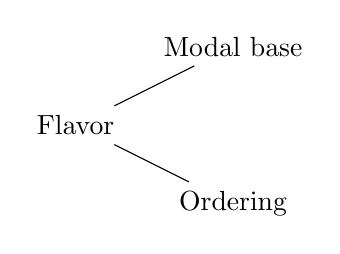
\begin{tikzpicture}[baseline=(current bounding box.north)]
    \node (f) at (0,0) {Flavor};
    \node (m) at (2,1) {Modal base};
    \node (o) at (2,-1) {Ordering};
    \draw (f) -- (m);
    \draw (f) -- (o);
  \end{tikzpicture}
}%
Kratzer famously proposed a different diagnosis: modals are \emph{doubly
  relative}, requiring two separate contextually supplied pieces of information.
In addition to the accessibility relation or \term{modal base} (a function that
assigns a set of accessible worlds to any evaluation world), modals are also
sensitive to an \term{ordering} of the accessible worlds.

\subsection{Mathematical interlude on orderings}
\label{subsec:math-orderings}

All order relations are binary relations between the elements of a set. Here
we're dealing with sets of worlds, but we can order soccer teams (by how good
they are), people (by how rich they are, or by how close to Rome they were
born), or race horses (by how they finished in the race). You get the idea.

In some sense, the most general kind of order is a \term{preorder}, one that you
could read as ``at least as highly ranked as''. It would be \term{reflexive},
since any element is trivially at least as highly ranked as itself. And it would
be \term{transitive}, since if $x$ is at least as highly ranked as $y$ and $y$
is at least as highly ranked as $z$, then surely $x$ is at least as highly
ranked as $z$.

When a preorder is also \term{anti-symmetric} (no distinct elements can have the
same rank), it is called a \term{partial order}. An order is \term{strict} if it
actually doesn't allow elements at the same rank, so it is transitive but
asymmetric. An order is \term{total} if it is a \term{complete} relation: any
two distinct elements are related in one way or the other.

An order is \term{well-founded} if for any subset of the domain of the relation,
there are elements in the subset that are ``optimal'': there is no other element
in the subset that is strictly better by the ordering. Any order on a finite set
is well-founded, but not every order on an infinite set is.

We provide two handy charts, one list of ours and one from Amartya Sen's
influential book \emph{Collective Choice and Social Welfare}
\parencite{sen-1970-collective-choice}.

\enlargethispage{36pt}
\begin{figure}[!htb]
  \centering
  \begin{tabular}{lp{19em}}
    \toprule[0.05em]
    \(R\) is \textbf{irreflexive} on \(S\) &
                                             \(\forall x\in S\colon \neg R(x,x)\)\\
    \(R\) is \textbf{reflexive} on \(S\) & \(\forall x\in S\colon R(x,x)\)\\
    \(R\) is \textbf{transitive} on \(S\) &
                                            \(\forall x,y,z\in S\colon R(x,y)\ \&\ R(y,z) \rightarrow R(x,z)\)\\
    \(R\) is \textbf{symmetric} on \(S\) &
                                           \(\forall x,y\in S\colon R(x,y) \leftrightarrow R(y,x)\)\\
    \(R\) is \textbf{antisymmetric} on \(S\) &
                                               \(\forall x,y\in S\colon R(x,y)\ \&\ R(y,x) \rightarrow x=y\)\\
    \(R\) is \textbf{asymmetric} on \(S\) &
                                            \(\forall x,y\in S\colon R(x,y) \rightarrow \neg R(y,x)\)\\
    \(R\) is \textbf{complete} on \(S\) &
                                          \(\forall x,y\in S\colon x \neq y \rightarrow R(x,y) \vee R(y,x)\)\\
    \(R\) is \textbf{dense} on \(S\) &
                                       \(\forall x,y\in S\colon x \neq y \conj R(x,y) \rightarrow\)\newline
                                       \hfill\(\exists z\in S\colon z \neq x
                                       \conj z \neq y \conj R(x,z) \conj
                                       R(z,y)\)\\
    \(R\) is \textbf{well-founded} on \(S\) & \(\forall S'\subseteq S\ \exists
                                              x\in S'\co\)\newline \hfill\(\neg\exists y\in S'\co
                                              R(y,x)\ \&\ \neg R(x,y)\)\\
    \bottomrule[0.05em]
  \end{tabular}
  \caption{Properties of relations}
  \label{fig:order-properties}
\end{figure}
%
\note{The first few chapters of Sen's book are worth reading. A semantic
  introduction to orders can be found in \cite{landman-1991-structures}. If
  you're curious about the mathematical aspects of this topic, we recommend
  \cite{davey-priestley-2002-lattices-order}.}%
\begin{figure}[!htb]
  \centering
  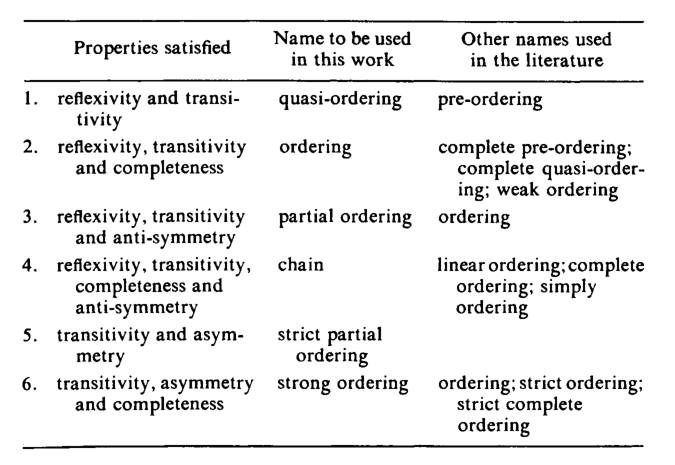
\includegraphics{./assets/sen-orders.pdf}
  \caption{\cite{sen-1970-collective-choice}'s summary of types of orders}
  \label{fig:sen-orders}
\end{figure}

\clearpage\subsection{Ordering worlds}
\label{subsec:ordering-worlds}

Armed with all this information we can return to the ordering of worlds. When we
think about worlds being ordered with respect to how well they obey a law, for
example, it's clear that we need to allow different worlds to be ``tied'', to be
at the same rank. So, our order will need to be a preorder. It's also wise not
to assume that for two given worlds, we can necessarily order them with respect
to each other at all. So, our order will not be total. %
\note{This is essentially the same as what is also known as the ``Limit
  Assumption'' in conditional/modal semantics. For discussion, see
  \cite{lewis-1974-dyadic} and now \cite{kaufmann-2017-limit}.}%
It will be a useful idealization if we assume that our orders will be
well-founded. Then, we can assume that we can always find worlds that are ``as
good as possible''. In sum, we assume that the context will supply a function
from evaluation worlds to a well-founded preorder on worlds. So, now we can find
for any set of worlds the contextually best worlds among them.

\note{Be aware that the literature is hopelessly inconsistent with respect to
  the direction of the symbols for ``at least as good as'' or ``better than''.
  Here, we use ``$w_{1}\le w_{2}$'' for ``$w_{1}$ is at least as good $w_{2}$''
  because the intuition is that $w_{1}$ is less far from the ideal than
  $w_{2}$.}%
Given a well-founded preorder $\le$, we define a function from sets of worlds to
subsets thereof that yields the $\le$-best worlds in the original set:

\ex For any set of worlds $p$ and any well-founded preorder $\le$ on $W$:\\
\hfill
$\opt_{\le}(p) = \{w\in p\co \neg\exists w'(w'\le w\ \&\ \neg(w\le w'))\}$
\xe

We can now state the semantics for doubly-relative modals. Here's the new entry
for \emph{must}:

\ex $\svt{must}^{w,g} = \lambda f_{s,st}.\ \lambda o_{s,sst}\co o(w)\text{ is a
  well-founded preorder on }W.\ \lambda p_{st}.$\\
  \hfill $\forall w'\in \opt_{o(w)}(f(w))\co p(w') = 1$
\xe
%
As before, the context supplies a flavor function $f$ that yields for any world
as set of $f$-accessible worlds. The context now also supplies a function that
for any world yields a well-founded preorder. We will call this function the
\textsc{ordering source} (a term from Kratzer). The semantics of modals uses the
preorder to order the set of accessible worlds and to find the best accessible
worlds. The modal \emph{must}, as a necessity modal, claims that all of the best
accessible worlds are worlds where its prejacent is true.

\begin{exercise}
  Write a doubly-flavored lexical entry for the possibility modal \emph{may}.
  \qed
\end{exercise}

Let's see how the analysis applies to \refx{ex:fine}: \emph{Howard has to pay a
  fine}.

\begin{itemize}
\item The modal base will be a function that assigns to any evaluation world the
  set of worlds where the same relevant circumstances hold. Since in our
  stipulated evaluation world, Howard failed to return his book, the modal base
  will assign to our world a set of worlds that only contains worlds where
  Howard didn't return the book.
\item The ordering source will be a function that assigns to any evaluation
  world an ordering that represents what the rules in that world prefer. For our
  cases and for the given evaluation world, the ordering will prefer worlds
  where no book is returned late to worlds where books are returned late. It
  further prefers worlds where fines are paid for late books to worlds where no
  fines are paid.
\item For our simple example then, any world in the modal base where Howard pays
  a fine will count as better than an otherwise similar world where he doesn't.
  The very best worlds simpliciter are worlds where there's never any
  late books, but since there aren't any such worlds in the modal base, the
  ordering has to make do with what it's given.
\item Modals then make quantificational claims about the best worlds in the
  modal base (those for which there isn't a world in the modal base that is
  better than them).
\item In our case, \refx{ex:fine} claims that in the best worlds (among
  those where Howard failed to return his book), he pays a fine.
\end{itemize}

\subsection{Kratzer's way}
\label{sec:kratzer-way}

As we've seen in the previous chapter, Kratzer actually calculates the set of
accessible worlds from a function of type $\type{s,\type{st,t}}$ (what she calls
a \emph{conversational background}). Recall that the construction is simple:
find the worlds where all the propositions in the set are true. The additional
power that comes with using sets of propositions remains essentially unused in
the case of modal bases. So, to simplify matters, we will stick with our earlier
assumption that the domain of modals is a set of worlds resulting from applying
a contextually supplied value of a pronoun of type $\type{s,st}$ to the
evaluation world.

\note{For our example about Howard's fine, we might imagine that for our
  evaluation world, the ordering source assigns a set of propositions that
  contains (among others) the following two propositions: (i) nobody returns
  books late, (ii) anybody who returns a book late pays a fine. It's crucial
  here that the second proposition is (vacuously) true when nobody returns books
  late.}%
For the ordering component of the doubly-relative semantics of modals, Kratzer's
construction is quite intuitive. We assume that the ordering source argument is
a function from evaluation worlds to sets of propositions. The idea is now that
such a set $\mathcal{P}$ of propositions can be used to order the worlds in the
modal base.

For any pair of worlds $w_1$ and $w_2$, we say that $w_1$ comes closer than
$w_2$ to the ideal set up by $\mathcal{P}$ (in symbols:
$w_1 <_{\mathcal{P}} w_2$), iff the set of propositions from $\mathcal{P}$ that
are true in $w_2$ is a proper subset of the set of propositions from
$\mathcal{P}$ that are true in $w_1$.

Here's a more precise derivation of the ordering procedure:

\ex For any set of propositions $\mathcal{P}$, we define a strict partial order
$<_P$:\\
    \(\forall w', w''\co w' <_P w''\) iff \\
    \hfill \(\forall p \in \mathcal{P} \left( w'' \in p \rightarrow w' \in p \right)
    \mbox{ and } \exists p \in \mathcal{P} \left( w' \in p \wedge w'' \not\in p
    \right)\)

$w'$ is better than $w''$ according to $\mathcal{P}$ iff all propositions in $P$
that hold in $w''$ also hold in $w'$ but some hold in $w'$ that do not also hold
in $w''$.
\xe

And of course, once we have such a strict partial order and we assume
well-foundedness, as before, we can define the selection function that gives us
the set of $<_{\mathcal{P}}$-best worlds from any set $X$ of worlds:

\ex
$\opt_{<_{\mathcal{P}}}(X) = \{w\in X\co \neg\exists w'(w'<_{\mathcal{P}} w)\}$
\xe

Finally, we need to rewrite the semantics of modals so that they are sensitive
both to a modal base/accessibility relation and an ordering source of the
Kratzerian kind:

\ex\label{ex:modal-2}
$\svt{must}^w = \lambda f_{s,st}.\lambda o_{s,stt}.\lambda p.\ \forall
w'\in\opt_{o(w)}(f(w))\co p(w)=1$.
\xe

\begin{exercise}
  Give an LF for the sentence \emph{Ashlyn must leave} that will work with the
  entry for \emph{must} in \Last. \qed
\end{exercise}

\subsection{More cases of modal ordering}
\label{subsec:more-ordering}

The combination of ``facts on the ground'' and ``doing the best with what we
have'' is pervasive in intensional constructions. We will discuss a succession
of brief case-studies but there's still much to explore.

\medskip

\textbf{How to get to Harvard Square.} Our initial example involved deontic modality. Next is the closely connected
case of goal-oriented or teleological modality. You want to get to Harvard
Square from MIT. This is your primary goal. You have secondary goals: to not
spend a lot of money and to stay reasonably safe. I say:

\ex You ought to take the Red Line. \xe
%
\note{In \cite{fintel-iatridou-2008-ought}, a \emph{three}-factor analysis is
  proposed, distinguishing technically between the primary goal and a secondary
  ordering source. There's further discussion in work by
  \citet{rubinstein-2012-thesis,rubinstein-2014-necessity-comparison}.}%
A two-factor analysis of \Last might look like this:

\begin{itemize}
\item The modal base is circumstantial. It assigns to the evaluation world a set
  of propositions describing the relevant circumstances. Imagine that for our
  world, the following facts are relevant: (i) you are in Kendall Square, (ii)
  you can get to Harvard Square on the Red Line, by taxi or Lyft, or on foot,
  (iii) the Red Line costs \$1.25, takes 10 minutes, and is safe, (iv) the
  taxi/Lyft costs \$10, is fast, and is safe, (v) walking is free, slow, and
  possibly unsafe this time of the night.
\item The ordering source describes your goals (often called a
  \emph{teleological} ordering source). Your relevant goals in our world are:
  (i) you get to Harvard Square, (ii) you pay less than \$2, (iii) you are safe.
\item What are the best worlds in the modal base according to the given ordering
  source? The worlds where you take the Red Line.
\item That's why it seems true to say \Last.
\end{itemize}

\textbf{The weakness of \emph{must}.} A more controversial application of the two-factor analysis is found in
\cite{kratzer-1991-modality}: she argues that apparently strong necessity modals
in their epistemic construal are actually weakened by ordering. Consider someone
who observes people coming into a windowless classroom with wet outer clothing.
They might say:

\ex It must be raining. \xe
%
Kratzer argues that what underlies \Last is a combination of an epistemic modal
base and an ordering source based on not completely exceptionless generalization
and assumptions. %
\note{The debate continues with \cite{lassiter-2016-must,
    delpinal-waldon-2019-epistemic-tension, fintel-gillies-2020-sgs}.}%
In more recent work, \cite{fintel-gillies-2010-mss} have argued
that any weakness in the meaning of \Last has to do with an ``evidential
signal'' (that the evidence for the prejacent is merely indirect) rather than a
lack of logical strength. 

\textbf{Wanting what's best.} Intriguingly, we can find the facts + ordering phenomenology in the semantics of
propositional attitudes as well, most clearly with bouletic attitudes like
\emph{want}. \cite{heim-1992-attitude} tells the story of someone who in her
dream scenario would not teach next semester but knows that she will have to.
She does have preferences on what week days to teach. So, she says:

\ex I want to teach Tuesdays and Thursdays next semester.\xe
%
\note{Heim herself gives a dynamic semantics analysis for attitudes that
  incorporates these insights. In later work, \cite{fintel-1999-npi} gives a
  static version of a two-factor analysis that is closely modeled after
  Kratzer's analysis of modals. See also
  \cite{rubinstein-2017-straddling} for a recent discussion.}%
In terms of the two-factor analysis, the idea here is that the accessibility
relation is ``doxastic'': the modal base contains the worlds compatible with the
agent's beliefs. In the case at hand, all worlds in that modal base have her
teach. The ordering is based on her preferences: among the worlds in the modal
base, she prefers the ones where she teaches Tuesdays and Thursdays.

\textbf{The Good Samaritan.} \cite{prior-1958-escapism} introduced the following
``Paradox of the Good Samaritan''. Imagine that someone has been robbed and John
is walking by. It is easy to conceive of a code of ethics that would make the
following sentence true:

\ex John ought to help the person who was robbed.\xe

In our previous one-factor semantics for modals, we would have said that
\Last says that in all of the deontically accessible worlds (those compatible
with the code of ethics) John helps the person who was robbed. Prior's point was
that under such a semantics, something rather unfortunate holds. Notice that in
all of the worlds where John helps the person who was robbed, someone was robbed
in the first place. Therefore, it will be true that in all of the deontically
accessible worlds, someone was robbed. Thus, \Last will entail:

\ex It ought to be the case that someone was robbed.\xe
%
It clearly would be good not make such a prediction.

The doubly-relative analysis of modality can successfully avoid this unfortunate
prediction. We conceive of \LLast as being uttered with respect to a
circumstantial modal base that includes the fact that someone was robbed. Among
those already somewhat ethically deficient worlds, the relatively best ones are
all worlds where John helps the victim.

Note that we still have the problematic fact that among the worlds in the modal
base, all are worlds where someone was robbed, and we would thus appear to still
make the unfortunate prediction that \Last should be true. But this can now
be fixed. For example, we could say that \emph{ought $p$} is semantically
defective if $p$ is true throughout the worlds in the modal base. This could
be a presupposition or some other ingredient of meaning. So, with respect to a
modal base which pre-determines that someone was robbed, one couldn't
felicitously say \Last.

Consequently, saying \Last would only be felicitous if a different modal base
is intended, one that contains both $p$ and non-$p$ worlds. And given a
choice between worlds where someone was robbed and worlds where nobody was
robbed, most deontic ordering sources would probably choose the no-robbery
worlds, which would make \Last false, as desired.

\subsection{Ordering in conditionals}
\label{subsec:ordering-conditionals}

\note{Even though Lewis' work appeared five years after Stalnaker's, it was
  independently developed. See \cite{arvan-2015-sprigge} and Fn.29 in
  \cite{starr-2018-sep-counterfactuals} for further details about the
  intellectual history of these ideas.}%
Historically, the use of an ordering of possible worlds in the semantics of
intensional operatores was first proposed by Stalnaker and Lewis in their work
on conditionals \parencite{stalnaker-1968-theory,lewis-1973-counterfactuals}. In
our attempt at an analysis for conditionals in Section~\ref{sec:conditionals},
we used a one-factor approach where conditionals quantify over \emph{all}
contextually accessible antecedent worlds. Stalnaker and Lewis argue that the
logic of conditionals, primarily counterfactuals, reveals the effects of an
ordering. %
\note{The match makes an early appearance in
  \cite{goodman-1947-counterfactual}.}%
Consider the case of a perfectly normal match in front of us and the following
two counterfactual conditionals:

\pex
\a If I had struck this match, it would have lit.
\a If I had dipped this match in water and struck it, it would have lit.
\xe
%
Intuitively, it is clear that \Last[a] may well be true while \Last[b] is almost
certainly false. But according to our previous analysis, which is a version of
what in the trade is called a ``strict conditional'' analysis, this cannot be.
If all of the accessible worlds where I strike this match are worlds where it
lights, then this must \emph{a fortiori} also be true of that subset of the
accessible worlds where I strike this match after having dipped it in water.

In the Stalnaker-Lewis ordering semantics, \Last[b] doesn't anymore follow from
\Last[a]. The most highly ranked worlds where I strike the match might well be
worlds where I don't dip it in water first, and so \Last[a] could be true while
\Last[b] is false.

Within this book's framework, we would replace the meaning for \emph{if} from
\refx{ex:if-strict-context-formal} in Section~\ref{sec:conditionals} with the
following two-factor meaning:

\ex
$\svt{if}^{w,g} = \lambda f_{s,st}.\lambda o_{s,stt}.\lambda p_{st}.\lambda
q_{st}.\ \forall w'\in \opt_{o(w)}(f(w) \cap p)\co q(w')=1.$
\xe
%
The crucial move here is that the antecedent proposition $p$ is used to find the
$p$-worlds that are among the $f$-accessible worlds. The resulting set of
accessible $p$-worlds is then ordered and the best accessible worlds $p$ are
what the universal quantifier makes a claim about.

But wait. In Section~\ref{sec:conditionals-modals}, we argued that
\emph{if}-clauses don't actually do their own modal quantification, so the
analysis in \Last can't be quite what we should adopt here. In fact, from the
restrictor point of view, the semantics of conditionals and their reliance on an
ordering on possible worlds should be a compositional effect: the
\emph{if}-clause serves as a restrictor for a (possibly covert) modal and it is
that modal that is sensitive to an accessibility relation and an ordering. In
the next section, we explore the interplay of conditionals and modals in a
theory that involves modal bases and orderings. Things are not entirely
straightforward. 

\section{The interplay of ordering and restricting}
\label{sec:interplay}

We return to Howard and the saga of the possibly late library book. Imagine that
we don't know whether he returned it late but we're confident we understand the
library regulations. So, we say:

\ex If Howard returned his book late, he has to pay a fine. \xe
%
\note{One might think that instead of starting with the worlds that match the
  evaluation world in whether the book was returned late, we could start with
  the worlds compatible with our evidence. Then, we would include both worlds
  where the book was late and where it wasn't. But even among those, the
  not-late worlds are the best. So, then again, the \emph{if}-clause could not
  find any antecedent worlds among the accessible worlds.} There is one analysis
that will not work: the restrictor analysis plus the pragmatically sophisticated
but semantically simple idea that modals are just sensitive to an accessibility
relation even when that relation incorporates considerations of ordering. So,
assume that the accessibility relation is the one that delivers the best worlds
among those that match the evaluation world with respect to whether the book was
late or not. Now, imagine a scenario where unbekownst to us, Howard actually
returned the book on time. It would seem that this would not threaten the
intuitive truth of \Last. But according to the analysis under consideration, we
predict something odd: the worlds that match the evaluation world are all worlds
where the book was not late and the best ones among them thus are also not-late
worlds (and of course they are worlds without a fine). The \emph{if}-clause
would then try to find late worlds in that set of accessible worlds, but since
there are none, we would get an empty set of worlds to quantify over, resulting
either in vacuous truth or some kind of infelicity. This is not correct.

The two-factor analysis (modal base $f$, ordering $o$) can help with the issue.
The idea is that the \emph{if}-clause does not restrict the $o$-best $f$-worlds
but restricts $f$ before $o$ enters into the picture. In other words, we posit
an LF like this one:

\ex
\begin{forest}
baseline,
sn edges,
for tree={s sep=5mm, inner sep=0, l=0}
[{}, my pretty nice empty nodes
[
[
[have to]
[
[$f_{3,\type{s,st}}$]
[
[if]
[[the book is late, roof]]
]
]
]
[$o_{5,\type{s,stt}}$]
]
[[Howard pays a fine, roof]]
]
\end{forest}
\xe
%
To evaluate this LF, we can use the entry for \emph{if} you developed in
Exercise~\ref{exe:if} and the entry for modals in \refx{ex:modal-2}. Note that
for the \emph{if}-clause not to be an idle restrictor, the worlds $f$ delivers
need to include worlds where the antecedent is true.

\begin{exercise}
  In fact, calculate the truth-conditions for \Last with the ingredients just
  mentioned. \qed
\end{exercise}

\begin{exercise}
  At this point, it would be very instructive to read
  \cite{kratzer-1991-modality}. In particular, you should study her version of
  the Samaritan Paradox in her Section 3.2 and her solution in her Section 8.
  \qed
\end{exercise}

\note{While Zvolensky's 2002 SALT paper was instrumental in bringing the issue
  into the natural language semantics literature, it had been already identified
  by \cite{frank-1996-dissertation} and in fact, it had been well-known as the
  ``if p, ought p'' problem in the more logico-philosophical world. See
  \cite{carr-2014-if-p-ought-p} for references and an important recent
  contribution.}%
It appears then that we have found vindication both for the two-factor semantics
for modals and for the restrictor theory. There's a problem though, illustrated
by \cite{zvolenszky-2002-problem} with the following example:

\note{As a matter of fact, Spears was paid to endorse Pepsi.}%
\marginfig{BritneyPepsi.png}%
\ex If Britney Spears drinks Coke in public, then she must drink Coke in public.
\xe
An intuitively plausible use case for \Last would be a situation where we
consider the possibility of seeing Spears drinking Coke in public. We conclude
that if we saw her drinking Coke, we would be able to deduce that she is somehow
contractually obligated to drink Coke.

Unfortunately, our current analysis predicts that \Last should, if anything, be
vacuously true rather than making a contingent claim. The \emph{if}-clause would
restrict whatever accessibility relation we're using and ensure that we're only
dealing with worlds where Spears drinks Coke in public. Then, the ordering would
apply to find the best such worlds. Finally, the modal would say that the best
such worlds are worlds where she drinks Coke in public. That is of course
trivially true.

Consider what is needed to make the modal claim (that Spears must drink Coke in
public) non-trivial. The domain of quantification needs to include worlds where
she doesn't drink Coke (perhaps she drinks Pepsi, or Poland Spring Water). Then,
the modal's ordering source identifies the best worlds and the modal says that
all of those are Coke worlds. This non-triviality can only arise if
\emph{if}-clause doesn't in fact restrict the modal to Coke worlds in the first
place. So, is the restrictor theory in trouble?

At this point, we must recall that under the restrictor theory,
\emph{if}-clauses can also restrict covert modals. This means that when we have
an \emph{if}-clause and an overt modal, we can't automatically conclude that the
conditional is restricting that modal. It might be restricting another
modal, a covert one, instead.

So, let's look at \Last in that light. Imagine that the \emph{if}-clause is
restricting a higher covert epistemic modal. Then, we are taken from the
evaluation world to those worlds compatible with our evidence where Spears
drinks Coke. We are saying that in all of those worlds Spears is obligated to
drink Coke. That will be a non-trivial claim if the worlds the lower modal
quantifies over contains both Coke and non-Coke worlds.

More technically, we'd be working with an LF like the one sketched in \Next. We
use $\Box$ for the covert modal. We need to distinguish four modal parameter
``pronouns''.

\ex
$\Box$ ($f_{1}$ if Coke) ($o_{1}$) [ must $f_{2}$ $o_{2}$ Coke ]
\xe
%
What values for the four parameter would yield the reading we want? $f_{1}$
should give us the worlds compatible with our evidence. $o_{1}$ could be trivial
or the kind of not entirely reliable evidence that \cite{kratzer-1991-modality}
argues for. Note that the higher modal will pass down only Coke-worlds.
Crucially, $f_{2}$ would give us both Coke and non-Coke worlds when applied to
the epistemically accessible worlds passed on by the higer operator. $o_{2}$,
finally, would encode Spear's contractual obligations.

\note{See \cite{geurts-2004-ambiguity} for a discussion of how this kind of
  structure is expected.}
With this, we have rescued the restrictor theory. The existence of such nested
structures is predicted by the framework and now we see that they are
empirically attested.  

Let's return to the case of Howard and his book again. As it turns out, we could
get the correct reading for our sentence \emph{If Howard returned the book late,
  he has to pay a fine} without having \emph{if} directly restrict the overt
modal. Assume that the \emph{if}-clause restricts a higher covert modal, again
maybe an epistemic one. And now, in contrast to the Spears example, assume that
the lower $f$-relation assigns to any of the worlds passed down (all of which
will be late book worlds) a set of worlds matching the facts about whether the
book was returned late. So, in effect, the conditional antecedent will end up
restricting both modals: the higher one directly and the lower one indirectly
since the lower accessibility relation will ensure matching of the relevant
fact.

This possibility led \cite{frank-1996-dissertation} to propose that deontic
modals in fact never are directly restricted:

\begin{quote}
  There are in fact no truly deontically modalized \emph{if}-conditionals.
  Instead, we assume conditionals with a deontic modal operator in the
  consequent clause to be analyzed throughout in terms of an implicit or
  explicit epistemically (or circumstantially) based modal operator. The deontic
  modal adverb is then to be analyzed within the scope of the `higher' epistemic
  modal operator.
\end{quote}

Now, if this is in fact feasible, why should we then still maintain the
restrictor analysis in the first place? Why not go back to the earlier idea that
\emph{if} is a modal operator in its own right? 

\marginfig{map.png}%
To evaluate this possibility, let's return once more to our friends who do not
know precisely where they are. Imagine that they have reason to think that among
the two Rte 117 possibilities, Stow is much more likely than Maynard, perhaps
because they know Maynard a bit better and think that if they were there, they
would very likely recognize some building or other. They have no reason to think
that Stow is more likely than Hudson (which is on Rte 62, remember). So, they
say:

\ex If we're on Route 117, we ought to be in Stow. \xe
%
Now, to be clear: they are still lost, so their evidence is compatible with them
being on either of the two routes and in any of the three towns. So, for \Last
to have a chance of being true, the modal \emph{ought} here can't simply map the
evaluation world to the worlds epistemically accessible from it (and then
potentially order the resulting worlds). We need to narrow things down to the
Route 117 worlds, even though our friends don't know whether they're there, even
if they are. So, as things stand, we still need the restrictor analysis. And we
need the restriction to happen \emph{before} the ordering applies. So, for now,
\Last provides the strongest argument we have for both the restrictor theory and
the two-factor semantics for modals.

At this point, we leave this intriguing and complex inquiry and refer you to the
ever-growing literature, some we've already mentioned and more we will list
below. 

\section*{Further readings} 

\textbf{Conditionals}. In-depth overviews of the logico-philosophical
perspective on conditionals include \cite{nute-1984-conditional},
\cite{edgington-1995-conditionals}, \cite{bennett-2003-guide}, and
\cite{starr-2018-sep-counterfactuals}.

Ideas pertaining to the implementation of the restrictor theory are found in
\cite{reich-2009-asymmetric} and \cite{ebert-ebert-hinterwimmer-2014-unified}.
\cite{schlenker-2004-conditionals} presents an alternative that is at least
plausibly in the same orbit. One should really take into account what we know
about the syntax of conditionals, some of which is discussed in Chapter 3 of
Kai's thesis but much more is found in \cite{bhatt-pancheva-2006-conditionals}.
\cite{rothschild-2011-conditionals-restrictors} explains the restrictor theory
to philosophers, might be useful as an additional reading.

\cite{gillies-2010-iffiness} proposes an ingenious alternative to the restrictor
theory. \cite{khoo-2011-gillies} files a complaint about the coverage of
Gillies' proposal. The interaction of conditionals with probability operators is
very tricky, see \cite{egre-cozic-2011-if-prob} and
\cite{fintel-gillies-2015-hedging} for some discussion.

\cite{higginbotham-1986-davidson} identified the interaction of negative
quantifiers like \emph{no student} with conditionals as a compositionality
puzzle. The restrictor theory has sometimes been seen as a solution to the
puzzle \citep{fintel-1998-qandif} and sometimes not
\citep{fintel-iatridou-2002-ifwhen}. See \cite{dekker-2001-if-only},
\cite{higginbotham-2003-conditionals}, \cite{leslie-2009-unless},
\cite{huitink-2010-quantified-conditionals}, \cite{klinedinst-2011-qc-cem},
\cite{kratzer-2015-hook}, \cite{lauer-nadathur-2016-qic-most} among others.

To understand \emph{only if}-conditionals, \cite{fintel-1997-bare} needs to work
hard to neutralize the universal force of bare conditionals stemming from
Kratzer's implicit necessity modal.

\cite{herburger-2015-only-if,herburger-2016-perfection}, and
\cite{bassi-bar-lev-2017-unified-existential} consider the possibility that
bare conditionals are actually (sometimes or always) existentially quantified.

\textbf{Attitudes}. Linguistic work on attitudes has often been concerned with
various co-occurrence patterns, particularly which moods (indicative or
subjunctive or infinitive) occur in the complement and whether negative polarity
items are licensed in the complement. Mood licensing: \cite{portner-1997-mood}.
NPI-Licensing: \cite{kadmon-landman-1993-any}, \cite{fintel-1999-npi},
\cite{giannakidou-1999-affective}.

Tamina Stephenson in her MIT dissertation and related work explores the way
attitude predicates interact with epistemic modals and taste predicates in their
complements: \cite{stephenson-2007-judge-lp,stephenson-2007-thesis}.

Jon Gajewski in his MIT dissertation and subsequent work explores the
distribution of the \term{neg-raising} property among attitude predicates and
traces it back to presuppositional components of the meaning of the predicates:
\cite{gajewski-2005-thesis,gajewski-2007-neg-raising}.

Interesting work has also been done on presupposition projection in attitude
contexts: \cite{asher-1987-attitudes}, \cite{heim-1992-attitude},
\cite{geurts-1998-attitudes}.

\textbf{Modals}. On the syntax of modals, there are only a few papers of uneven
quality: \cite{bhatt-1997-haveto}, \cite{wurmbrand-1999-raising},
\cite{cormack-smith-2002-modals}, \cite{butler-2003-modality}. Follow up on
older references from the bibliographies in these papers. The following paper
explores some issues in the LF-syntax of epistemic modals:
\cite{fintel-iatridou-2003-ec},

Valentine Hacquard's MIT dissertation is a rich source of
cross-linguistic issues in modality, as is Fabrice Nauze's Amsterdam
dissertation: \cite{hacquard-2006-dissertation},  \cite{nauze-2008-thesis}.

Some more recent work by Hacquard deals with deriving and correlating modal
flavors with syntactic position of the modal auxiliaries:
\cite{hacquard-2010-event-relativity}, \cite{hacquard-2013-modality}. A recent
handbook article by Hacquard on actuality entailments (involving the interaction
of modality with aspect; we'll discuss aspect later in these notes):
\cite{hacquard-2016-actuality}.

The semantics of epistemic modals has become a hot topic recently. Here are some
of the main references: \cite{hacking-1967-possibility},
\cite{teller-1972-epistemic}, \cite{derose-1991-epistemic},
\cite{egan-hawthorne-weatherson-2005-epistemic}, \cite{egan-2007-epistemic},
\cite{macfarlane-2006-might}. \cite{stephenson-2007-judge-lp},
\cite{hawthorne-2007-danger}, \cite{fintel-gillies-2008-cia-leaks},
\cite{fintel-gillies-2008-mmr}.

A paper by Pranav Anand and Valentine Hacquard tackles what happens to epistemic
modals under attitude predicates:
\cite{anand-hacquard-2013-epistemics-attitudes}.

Evidentiality is a topic closely related to epistemic modality. Some references:
\cite{willett-1988-evidentials}, \cite{aikhenvald-2004-evidentiality},
\cite{drubig-2001-epistemic}, \cite{blain-dechaine-2007-evidentials},
\cite{mccready-ogata-2007-evidentials}, \cite{speas-2008-evidentials},
\cite{fintel-gillies-2010-mss}.

Modals interact with disjunction and indefinites to generate so-called
\term{free choice}-readings, which are a perennial puzzle. Here is just a very
small set of initial references: \cite{kamp-1973-freechoice},
\cite{zimmermann-2000-fc-disjunction}, \cite{schulz-2005-fcp-synthese},
\cite{aloni-2007-freechoice}, \cite{alonso-ovalle-2006-thesis},
\cite{fox-2007-freechoice}, \cite{rooij-2006-donkeys}.

\textbf{Restricting and ordering}. Very important for the problem we ended the
chapter on are these papers:
\cite{kaufmann-schwager-2009-conditional-imperatives} and
\cite{condoravdi-lauer-2016-anankastic}. 

%%% Local Variables:
%%% mode: latex
%%% TeX-master: "ik-book"
%%% End:
